\documentclass[10pt, a4paper, conference, onecolumn]{IEEEtran}
\IEEEoverridecommandlockouts
% The preceding line is only needed to identify funding in the first footnote. If that is unneeded, please comment it out.
\usepackage[T1]{fontenc}
\usepackage{lmodern}
\usepackage{cite}
\usepackage{IMTtikz}
\usepackage[hidelinks,colorlinks=true,urlcolor=blue,linkcolor=black,citecolor=blue]{hyperref}

\usepackage{polyglossia}

\setdefaultlanguage[variant=brazilian]{portuguese}
\SetLanguageKeys{portuguese}{indentfirst=false}

\usepackage[brazilian]{cleveref}
\crefformat{footnote}{#2\footnotemark[#1]#3}

\setotherlanguages{english}
\SetLanguageKeys{english}{indentfirst=false}

\usepackage{algorithmic}
\usepackage{multicol,multirow,makecell}
\usepackage{caption}
% \usepackage{listings}
\usepackage{graphicx}
\usepackage{float}
\usepackage{textcomp}
\usepackage{xcolor}
\usepackage{booktabs}

\captionsetup[table]{skip=10pt}

\def\BibTeX{{\rm B\kern-.05em{\sc i\kern-.025em b}\kern-.08em
    T\kern-.1667em\lower.7ex\hbox{E}\kern-.125emX}}

\usepackage[stretch=10,shrink=10]{microtype}
\AtBeginEnvironment{verbatim}{\microtypesetup{activate=false}}

% IEEE specific names
\def\IEEEkeywordsname{Palavras-chave}
% \def\IEEEproofname{Proof}

\usepackage{fancyvrb}
\VerbatimFootnotes

\begin{document}

\title{\textbf{Projeto de Pesquisa para Iniciação Científica} \\
{Comparando a utilização de soluções livres e proprietárias para programação geral de GPUs}
% \thanks{Identify applicable funding agency here. If none, delete this.}
}

\author{\IEEEauthorblockN{Isabella Basso do Amaral} \\
\and
\IEEEauthorblockN{Orientador: Alfredo Goldman Vel Lejbman}
\IEEEauthorblockA{\textit{Instituto de Matemática e Estatísica} \\
\textit{Universidade de São Paulo}\\
São Paulo, Brasil \\
\texttt{\href{mailto:gold@ime.usp}{\nolinkurl{gold@ime.usp}}}}
}

\maketitle

\begin{abstract}
    A adoção, por parte da comunidade científica, de \textit{software} com
    intuito de aproximar soluções para problemas relevantes no cenário
    contemporâneo traz consigo desafios além dos técnicos, principalmente, no
    que diz respeito à utilização de soluções livres para a execução de tais
    pesquisas.
    Esta é essencial para que não violemos princípios básicos da pesquisa
    científica como a entendemos nos dias de hoje, como por exemplo o princípio
    da reprodutibilidade.
    No presente projeto, então, verificamos a distribuição de pesquisas em
    relação à sua utilização de soluções livres ou proprietárias,
    especificamente no contexto de \textit{GPU General Programming} (GPGPU),
    assim como as disparidades entre opções livres e proprietárias que
    complexificam o cenário ideal.
    Munidos desses dados, buscaremos uma compreensão mais aprofundada da
    situação, tomando em consideração aspectos técnicos de cada alternativa.
    A partir deste ponto, exploramos os passos necessários para facilitar a
    adoção de soluções livres, assim como o seu desenvolvimento.
\end{abstract}

\begin{IEEEkeywords}
    APIs gráficas, GPU, CUDA, Vulkan, Compute, OpenCL, FLOSS, código proprietário
\end{IEEEkeywords}

\section{Introdução}

O computador tornou-se parte indispensável da pesquisa acadêmica principalmente
``resolvendo'' (aproximando) problemas numéricos, os quais são, em grande
maioria, insolúveis sob o olhar analítico.

A aproximação de soluções para problemas numéricos em \textit{software}, embora
não seja uma questão nova ou sequer teórica, demanda a utilização de técnicas
avançadas de programação exigindo, por vezes, o uso de \textit{software}
extremamente particular, complexo e que demanda conhecimento técnico
específico, tanto da teoria quanto do \textit{software} em questão.

\subsection{Otimização}

Também no que diz respeito aos problemas numéricos, gostaríamos de ressaltar,
em especial, a possibilidade de paralelizá-los, agilizando (por vezes
desproporcionalmente) a produção de resultados. Em diversos casos, tais
otimizações são necessárias para que possamos produzir resultados
oportunamente, levando em conta simplesmente a capacidade de paralelização do
\textit{hardware} moderno \textit{versus} suas capacidades de execução linear.

A métrica utilizada para a capacidade de um dado \textit{hardware} no contexto
de aplicações numéricas é a quantidade de operações de ponto flutuante que
podem ser executadas por segundo [FLOPS] (\textit{floating point operations per
second}) -- veja \cite{dolbeau2018theoretical, sun2019summarizing} para uma
discussão aprofundada sobre essa métrica e sua relevância na computação
moderna.

Notamos que, com frequência, o \textit{hardware} moderno é muito mais eficiente
em tarefas que aproveitam sua capacidade de paralelização
\cite{doi2018performance} -- não necessariamente aumentando por um fator linear
em relação à disponibilidade de recursos (nesse contexto lidamos com
\textit{cores} ou \textit{threads}\footnote{ Para uma discussão extensiva sobre
o papel de cada um desses recursos, veja \cite{magro2002hyper}. }), pois
existem diversos fatores a serem levados em conta como, por exemplo,
concorrência\cite{zhou2005improving}.

A GPU (\textit{Graphics Processing Unit}) é um componente especializado em
tarefas de paralelização, de tal forma que, atualmente, é utilizada
extensivamente para auxiliar na resolução de problemas nas áreas de física,
biológia, química e até mesmo da matemática moderna sendo, por vezes, mais
relevante do que a CPU (\textit{Central Processing
Unit}) de um dado sistema em aplicações como aquelas
da ciência de dados\cite{buber2018performance}.

\subsection{Sobre o uso de \textit{software} livre em aplicações científicas e sua importância}\label{sec:soft-livre}

No que tange a utilização de \textit{software} para aplicações científicas, nos
preocupamos principalmente com a utilização de \textit{software} livre, que,
estritamente falando, é aquele que se alinha perfeitamente com os princípios da
pesquisa científica.

Chamamos de \textbf{\textit{software} livre} (abreviado por FLOSS ou FOSS em
inglês) aquele que é aberto para ser lido e auditado, e que não depende de
corporações (embora possa ser auxiliado por estas) para que se mantenha.
Possuíndo comunidades autonomas de usuários e desenvolvedores que o mantém de
acordo com interesses pessoais e plurais, porém não necessariamente sem o
envolvimento de capital.

O \textit{software} livre permeia todo o contexto computacional moderno, sendo
utilizado extensivamente na internet (e.g. $\approx \qty{80}{\percent}$ dos
servidores utilizam \textit{Linux} \cite{w3techs}), no contexto do
desenvolvimento de \textit{software} e, especialmente, na pesquisa científica.

Contrastamos tal com o \textbf{\textit{software} proprietário}, onde a
contribuição de um indivíduo sempre será atrelada com interesses corporativos
pois pertence à uma empresa e é secreto sendo, portanto, impossível auditá-lo.

Existe ainda o \textit{superset} de \textit{software} livre, que é o
\textbf{\textit{software} aberto}, onde pode existir uma empresa que o mantém
de acordo com seus interesses, porém este não é secreto, podendo ser auditado e
aceitando contribuições individuais\footnote{
    No presente projeto, no entanto, vamos nos dedicar exclusivamente à
    problemática do \textit{software} livre \textit{versus} \textit{software}
    proprietário.
}.

Note, então, que a utilização de \textit{software} livre é preferível no
contexto científico, pois soluções proprietárias demandam desmedida confiança a
interesses corporativos, podendo causar conflitos de interesse tácitos e indo
de encontro a princípios da ciência como a temos hoje, onde reprodutibilidade e
transparência são essenciais.

Com isso em mente, advogamos pelo uso do \textit{software} livre nesse contexto
o que, infelizmente, ainda não é totalmente plausível como será explorado mais
a frente.

\section{Justificativa}

Haja vista que a GPU é um componente de \textit{hardware} sendo, então,
necessário comandá-la de forma específica e precisa, idealmente gostaríamos de
abstrair detalhes do \textit{hardware} específico, de tal forma que tenhamos
fino controle sobre sua utilização, sem comprometer, porém, seu desempenho
(i.e. a abstração deve otimizar o que quer que seja tendo em mente o
\textit{hardware} específico).

\subsection{Compiladores} \label{sec:compiladores}

Classicamente, utilizamos \textit{shaders} para a programação de GPUs, sendo
mais ou menos análogos à programação de CPUs em sua sintaxe, mas não
necessariamente em sua lógica, o que torna seu uso não-trivial para alguém sem
o conhecimento específico. O código do \textit{shader} é compilado em
etapas, sendo primeiramente convertido para uma linguagem intermediária, onde é
otimizado com base em conceitos primitivos próprios para abordagens de
paralelização. Depois, sendo convertido para um binário otimizado para a GPU
específica onde será executado, e então enviado para o \textit{hardware}, como
ilustrado na \ref{fig:mesa-cs}.
No contexto geral do Linux, essa é apenas uma pequena parte do processo de
execução de um \textit{shader}, o que podemos ver na \ref{fig:linux-gs}.

\begin{multicols}{2}
    \begin{figure}[H]
    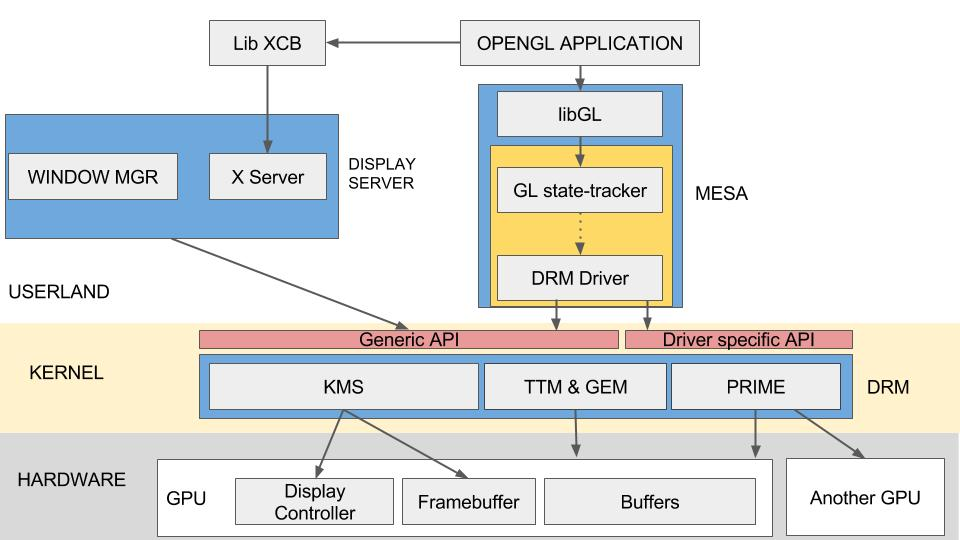
\includegraphics[width=\linewidth]{linux-stack.jpeg}
    \caption{\textit{Stack} gráfica utilizada em sistemas operacionais baseados
        no \textit{kernel} Linux.}
    \label{fig:linux-gs}
    \end{figure}
    
    \columnbreak

    \begin{figure}[H]
    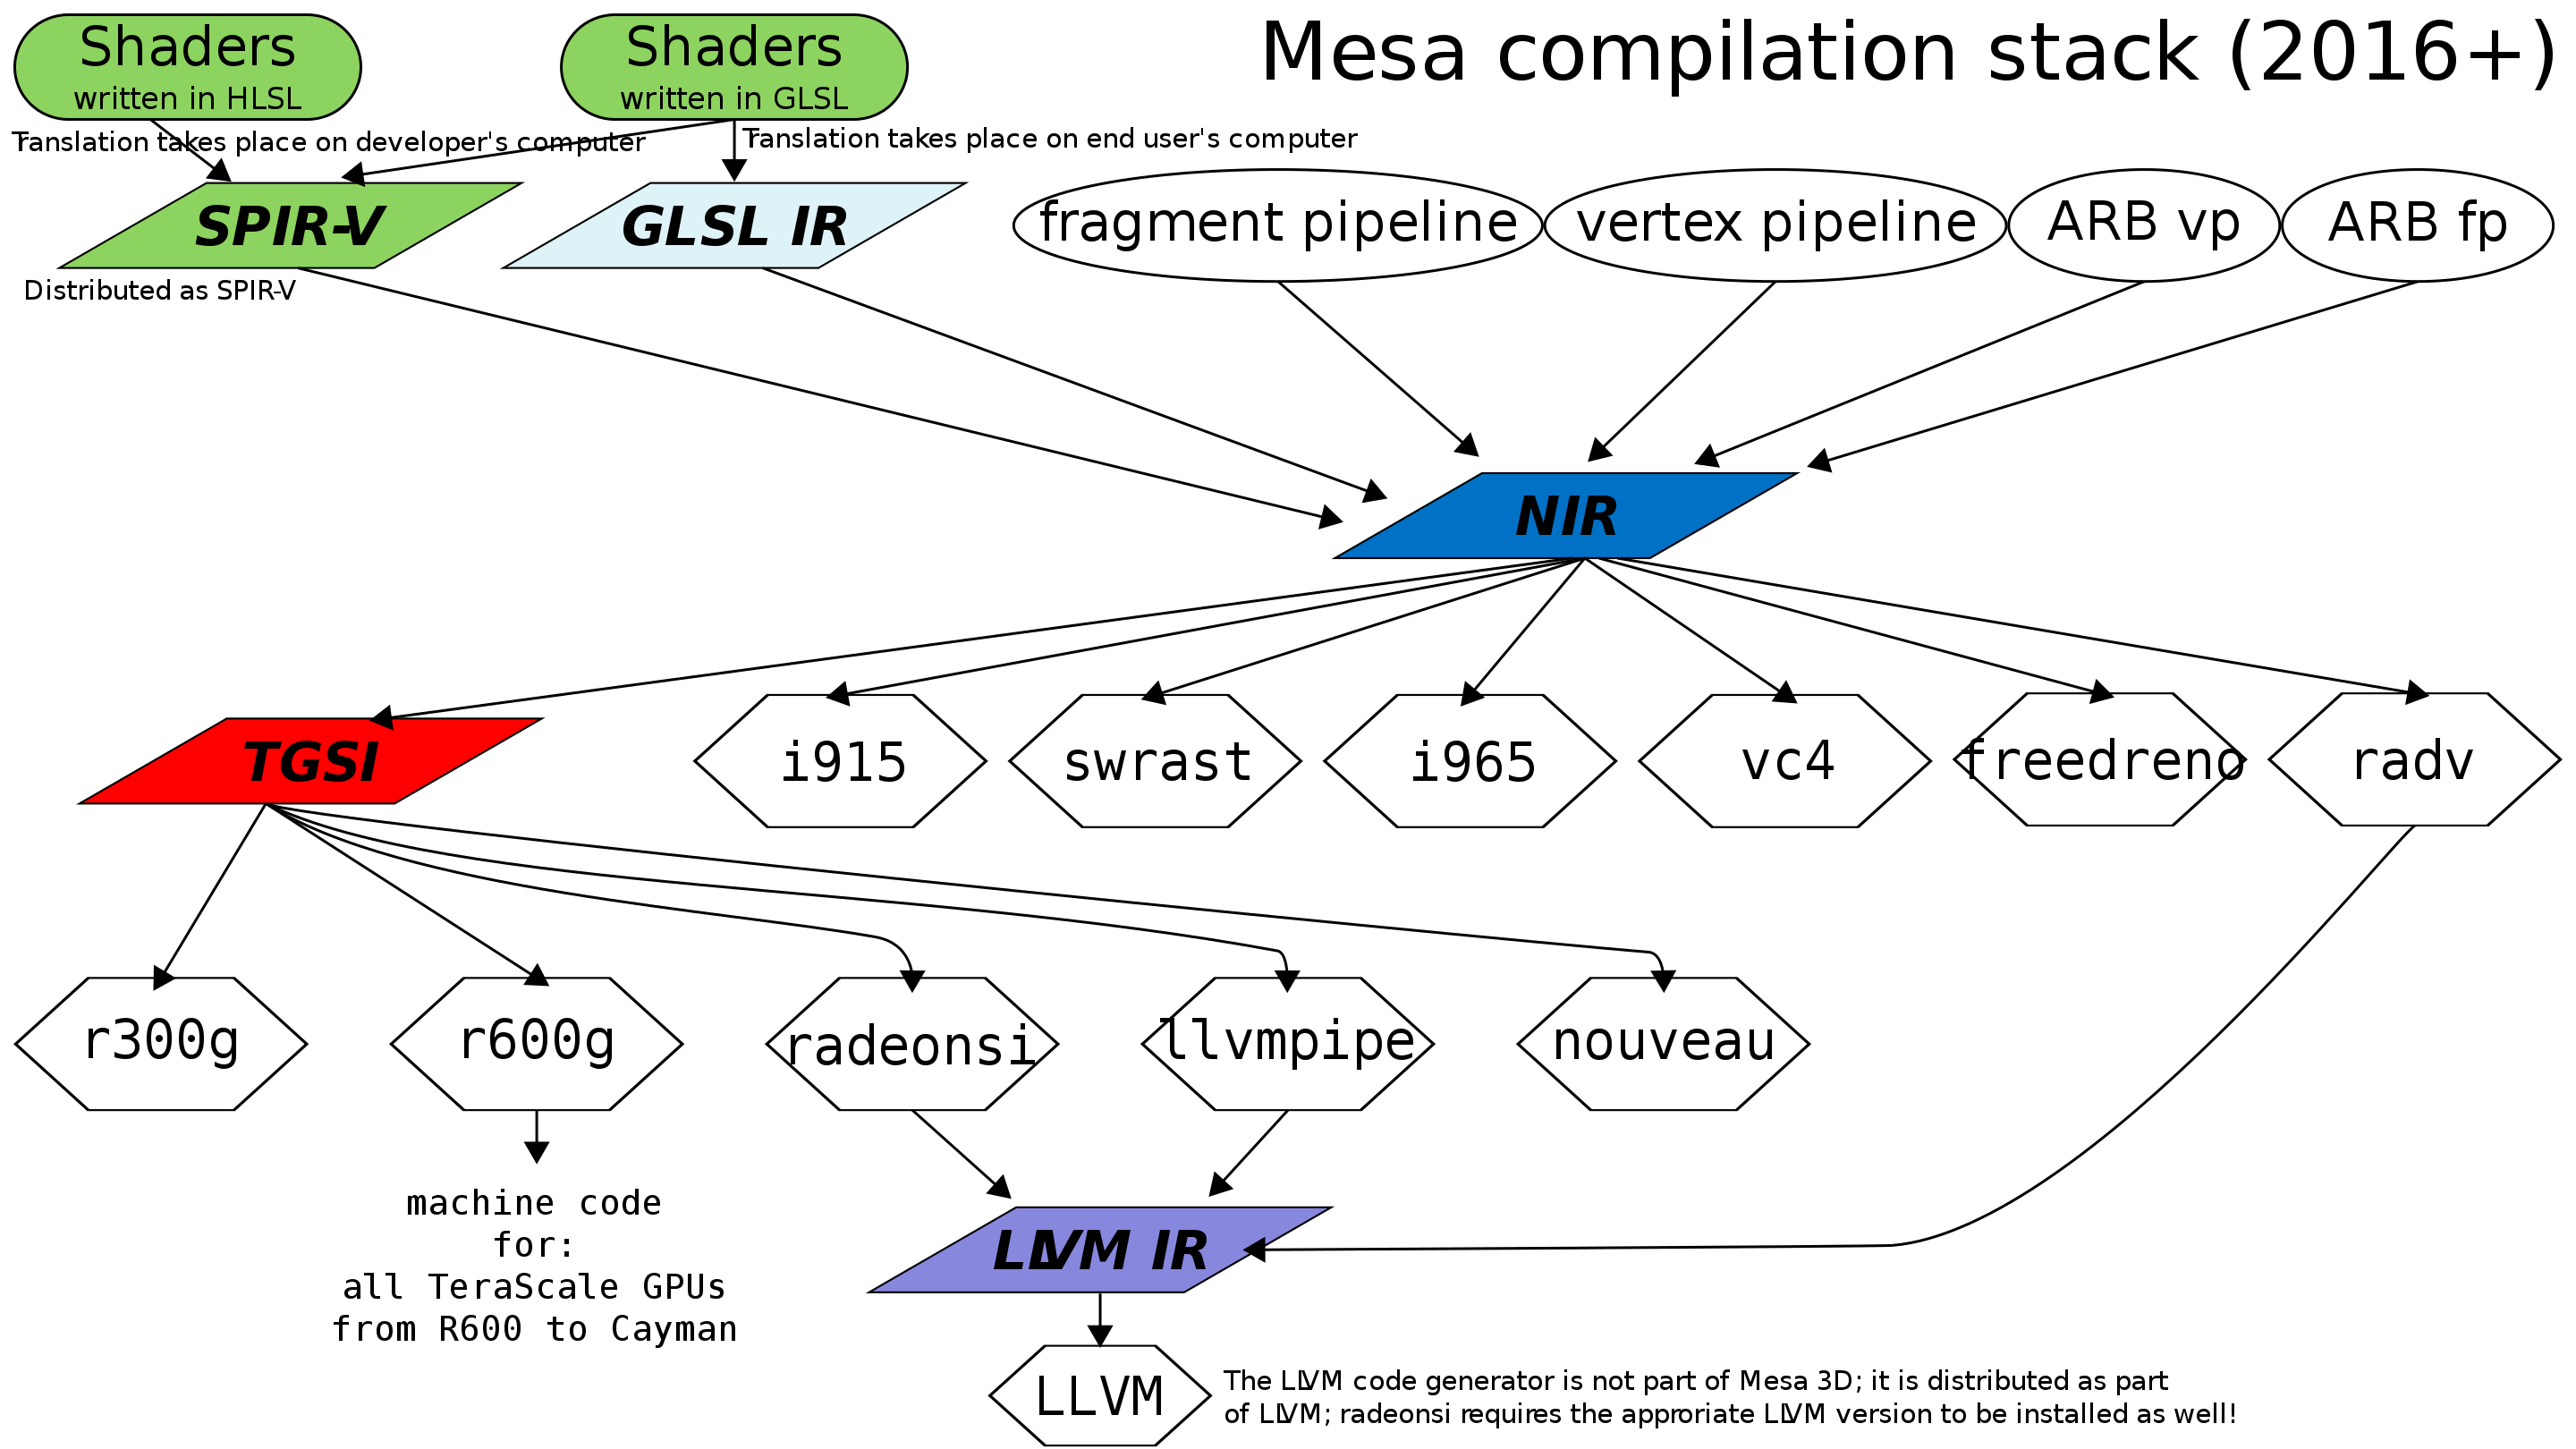
\includegraphics[width=\linewidth]{mesa.png}
    \caption{\textit{Stack} mais recente de compilação utilizada pelo Mesa, um
        \textit{software} responsável por APIs gráficas de código aberto no
        Linux. O Mesa recebe o código de um \textit{shader} a ser processado,
        executando os passos descritos acima (\ref{sec:compiladores}).}
    \label{fig:mesa-cs}
    \end{figure}
\end{multicols}

\subsection{Comparando o \textit{software} livre com o proprietário para aplicações científicas}

No contexto específico de aplicações numéricas, no presente projeto nosso
interesse é voltado à \textbf{programação geral} com GPUs (GPGPU), onde temos
utilização extensiva da linguagem \textbf{CUDA}, desenvolvida pela empresa
NVIDIA -- uma pioneira em computação gráfica.

A \textit{stack} (conjunto de \textit{software} e/ou \textit{hardware}) necessária
para a utilização do CUDA é, infelizmente, integralmente proprietária, desde a
implementação de sua API (\textit{aplication programming interface}), que é a
interface pela qual desenvolvedores podem acessar um dado conjunto de
funcionalidades, até os \textit{drivers} necessários para a execução do
\textit{software}. Algumas alternativas como o \textbf{OpenCL} ou o
\textbf{Vulkan} têm se tornado cada vez mais populares, porém é necessário
notar que o seu uso não implica em uma \textit{stack} livre, já que os
\textit{drivers} utilizados podem ser proprietários -- e.g. OpenCL + NVIDIA
implica que teremos que usar os \textit{drivers} proprietários da fabricante,
porém se usamos uma GPU da fabricante AMD, podemos utilizar \textit{drivers}
livres.
No presente projeto então, focamos estritamente nas APIs, já que os
\textit{drivers} envolvem uma camada espessa de abstrações, dificuldades e
tecnicidades muito além do escopo e do tempo planejado para o projeto.

Dada sua simplicidade e abrangência, o CUDA segue invicto em aplicações
científicas que utilizam GPUs -- essa afirmação infelizmente carece de fontes
acadêmicas, porém, assumindo que a proporção de projetos abertos\footnote{
    \label{footnote:cuda-github}
    Note que estes projetos não necessariamente são utilizados em pesquisas científicas,
    tomamos o número como base de referência para GPGPU genérica, o que inclui
    tais aplicações, e que muito provavelmente adotam ainda mais fortemente o
    uso de CUDA.
} (a maioria
dos quais está disponível no \href{https://github.com}{GitHub}) que utilizam
uma dada tecnologia para projetos fechados é a mesma, podemos realizar uma
busca simples no site:

\begin{itemize}
    \item Utilizando a barra de pesquisa, buscamos por CUDA, e filtrando por
        linguagem\footnote{
            A consulta específica utilizada nesse caso foi
            \verb|cuda language:cuda language:c language:c++ start:>=5 followers:>=5|
            de tal forma que apenas os projetos com mais de 4 seguidores e mais
            de 4 estrelas foram mostrados, além de utilizarem qualquer uma das
            3 linguagens (C, C++, CUDA). Esses filtros foram utilizados para
            vermos projetos minimamente relevantes.}
        encontramos projetos que de fato utilizam a tecnologia
        (1669 resultados).
    \item Repetimos o processo\footnote{
        Nesse caso, retiramos a linguagem CUDA dos resultados.
    }, porém buscando por OpenCL (647 resultados) e Vulkan (798
        resultados)\footnote{
            Note que, nesse caso, é impossível selecionar somente projetos
            relacionados à GPGPU, pois muitos destes não incluem essa
            palavra-chave, ou o termo correto (\textit{Vulkan Compute}).
        }.
    \item Estimando que a busca pelo termo ``Vulkan'' retornou 2/3 de
        resultados errados, já que ele é utilizado majoritariamente em
        aplicações que não se tratam de GPGPU, temos $ 1669 / (647 + 798/3 +
        1669) \gtrsim \qty{64}{\percent} $\cref{footnote:cuda-github} dos
        resultados utilizando CUDA (não necessariamente exclusivamente).
\end{itemize}

Notamos então, que a disponibilidade de alternativas livres (e viáveis) é de
grande importância de grande importância para a comunidade científica
contemporânea, como discutido em \cref{sec:soft-livre}.

% \begin{figure}[h]
%     \centering
%     \includegraphics[width=0.5\textwidth]{figures/cuda.png}
%     \caption{Comparação entre o \textit{software} livre e o proprietário para aplicações científicas}
%     \label{fig:cuda}
% \end{figure}

\section{Objetivos} \label{sec:objetivos}

Dada a utilização (aproximada) do CUDA em relação a alternativas livres,
possuímos diversos questionamentos que devem ser abordados no presente projeto,
como:

\begin{enumerate}
    \item\label{obj1} Qual a figura exata da adoção de \textit{software} livre para aplicações científicas?
    \item\label{obj2} Onde o CUDA se sobressai em comparação com essas alternativas?
    \item\label{obj3} Como podemos diminuir essa diferença e como facilitar a migração para soluções que usam exclusivamente código livre?
    \item\label{obj4} O cenário ideal é factível?
\end{enumerate}

Escolhemos o \textbf{OpenCL} e o \textbf{Vulkan} como objetos de análise nesse
projeto.
Ambos são fruto de específicações construídas pelo consórcio Khronos Group, do
qual 170 organizações são parte e que desenvolve diversas outras especificações
amplamente adotadas possuindo, portanto, um grande impacto na computação
moderna.
Implementações específicas de ambas especifícações serão escolhidas para uso
durante o projeto, a fim de realizarmos aperfeiçoamentos e comparações.

Uma das possibilidades de aplicação real do presente projeto no futuro é
procurar formas de se integrar o software livre disponível para GPGPU em
projetos livres de maior porte como o DemiKernel \cite{zhang2019m, zhang2021demikernel}.

\section{Cronograma}

\begin{table}[H]
    \centering
    \begin{tabular}{c c l c c} \toprule
        Semestre & Código & Nome & Pós-graduação & Carga horária \\ \midrule
        \multirow{2}{*}{2022.2} & MAC0344 & Arquitetura de Computadores & não & 4 A \\
                                & MAC0414 & Autômatos, Computabilidade e Complexidade & não & 4 A \\ \midrule
        \multirow{2}{*}{2023.1} & MAC5752 & Introdução à Computação Paralela e Distribuída & sim & 4 A + 2 P + 4 E \\
                                & MAC5743 & Sistemas Operacionais & sim & 4 A + 2 P + 4 E \\ \midrule
        \multirow{2}{*}{2023.2} & MAC5716 & Laboratório de Programação Extrema & sim & 4 A + 2 P + 4 E \\
                                & MAC5717 & \makecell[l]{Laboratório Avançado de Métodos \\ Ágeis de Desenvolvimento de Software} & sim & 4 A + 2 P + 4 E \\ \midrule
                         2024.1 & PCS3866 & Linguagens e Compiladores & não & 4 A \\ \bottomrule
    \end{tabular}
    \caption{Cronograma de disciplinas do projeto de avançado. Note que ``A''
    representa a carga horária de aulas, ``P'' representa a carga horária de
    projeto e ``E'' representa a carga horária de estudos da disciplina em
    questão.}
    \label{table:cronograma}
\end{table}

Além do que foi listado, também deverão ser feitos cursos extra-curriculares
da NVIDIA, com intuito de aperfeiçoar o conhecimento a respeito de CUDA, para
que possamos entender melhor suas vantagens e usos com relação às alternativas
que serão abordadas.

\section{Metodologia}

Tendo em mente os objetivos pontuados na \cref{sec:objetivos}, devemos começar
estudando formas de contabilizar a quantidade de aplicações científicas que
fazem uso de APIs gráficas livres e proprietárias (\cref{obj1}), assim como as
principais capacidades de cada uma e compará-las contra os casos de uso das
principais áreas de estudo das ciências (\cref{obj2}).
Essa etapa deve ser realizada no primeiro semestre do projeto (2022.2), enquanto
os temas de arquitetura de computadores e a base teórica para compilação são
introduzidos nas disciplinas respectivas (MAC0344 e MAC0414).

A arquitetura de computadores é importante pois desejamos entender aspectos de
otimização íntrinsecos à parte física desses sistemas complexos, para que assim
seja possível implementar soluções viáveis para aplicações científicas (que
requerem performance), e também úteis para a comunidade de usuários em geral.

Após adquirir esses dados e um conhecimento básico dos sistemas em questão,
estudaremos a paralelização e sistemas operacionais nas disciplinas respectivas
(MAC5752 e MAC5743), onde será desenvolvida um conhecimento mais específico das
implementações necessárias no contexto de GPGPU, além do contexto global onde
são executados.
Nesse momento, começamos a explorar possibilidades de melhorias das APIs livres,
primeiramente entendendo o que existe atualmente (i.e. estudando seu código) e
depois conversando com a comunidade sobre o que seria mais útil ou mais viável
dado a duração do projeto.

Por fim, devemos implementar as diversas melhorias fixadas anteriormente, o que
poderá ser feito em até um ano de projeto, e pode abranger também a integração
de ferramentas livres de GPGPU com outros projetos de interesse (veja a
\cref{sec:objetivos} \textsection 3 e/ou \cite{zhang2019m, zhang2021demikernel}).
Nesse contexto, as disciplinas de programação extrema e métodos ágeis
(respectivamente MAC5752 e MAC5743) serão de grande utilidade a fim de se
produzir código de qualidade e com metodologia.
Além disso, a disciplina de métodos ágeis possui um rico histórico com relação
ao \textit{software} livre, sendo o berço do grupo de extensão de código livre
na USP (\href{https://flusp.ime.usp.br/}{FLUSP}).
Também serão utilizadas algumas referências bibliográficas como
\cite{aniche2022effective, narayan2008structure, fowler2018refactoring,
arpaci2018operating, ritchie1978c, stroustrup2013c++}, para que possamos
embasar a metodologia de desenvolvimento de software.
Ao final do projeto (2024.1) a disciplina de compiladores servirá como
concretização dos conhecimentos adquiridos em MAC0414, de tal forma a
fornecer o panorama completo dos aspectos práticos da otimização do
\textit{software} a ser desenvolvido, nos permitindo aperfeiçoar o que fora
desenvolvido até então.

\bibliographystyle{IEEEtran}
\bibliography{../IEEEabrv,references}

\end{document}
